\chapter{绪论}{Introduction}
\section{研究背景和意义}{Background and Research Significance}
智慧城市是由数字城市、物联网和云计算三大类支撑技术组成,其中数字城市是智慧城市的核心,
主要包含天地空一体化空间信息快速获取、海量空间数据管理、空间信息可视化技术、空间数据分析挖掘和
网络服务技术\cite{李德仁2013智慧地球时代测绘地理信息学的新使命}。互联网尤其移动互联网的快速发展,
使得数字城市面临巨大的挑战:空间数据获取手段不再局限于传统人工测量,基于用户地理位置服务(Location Based Service, LBS)
功能使得网络中包含了用户的空间数据;每天产生的海量数据对数据存储、索引和查询提出高性能要求;
海量空间数据使得空间知识愈发贫乏,急需海量空间数据挖掘相关研究。

相关调查表明,中国大陆是全球移动互联网用户最多的地区,移动互联网设备上各种APP记录了每个用户生活的
方方面面,比如打车软件记录城市居民出行数据,O2O软件反映了城市线下商圈服务区域情况。其中以新浪微博为代表
的社交网络应用最为值得研究,超过一大半移动互联网用户都拥有新浪微博账号。作为高频使用应用程序,
新浪微博已经成为数字城市空间数据不可忽视的重要数据来源。在社交网络中,用户的行为往往是自发进行的,这些数据蕴含了城市居民
生活的真实信息,快速精确的对这些数据进行空间书分析和挖掘对智慧城市建设有着重大意义,主要包含
以下三个方面:

(1)对个人而言,对网络空间数据挖掘,可以发现不同的知识,为生活带来便利,如交通路线规划、旅游景点推荐等,构建城市智慧生活。

(2)对商业公司而言,通过空间数据挖掘发现目标客户使用习惯或群体性活动规律,对商业推广计划提出指导性意见,如广告投放、精准营销等,
是城市智慧商业重要组成部分。

(3)对政府决策部门而言,城市居民的社交网络中的行为是社会现实现象的反映,能够发现社会的经济、文化、交通等众多方面活动规律。为智慧城市
发展的各项决策提供建议。

智慧城市提出了海量空间数据高效处理的需求,目前针对海量数据普遍采用分布式并行计算,其核心思想是将海量数据划分
为若干个子集,将每个子集分配给不同的线程、进程或者是机器进行并行处理,最后将每个子集计算出来的结果进行合并,得到全局计算结果。
Hadoop MapReduce\cite{Shvachko2010The}是业界广泛使用的并行分布式计算框架,通过对数据处理过程的高度抽象,
使普通开发人员编写分布式并行计算成为可能。但是现实业务需求的更迭,这些计算框架面对迭代计算需求显得捉襟见肘,
Spark作为新一代的开源通用并行计算框架\cite{Zaharia2010Spark},大大扩展了MapReduce表现能力,
而且通过内存计算独特的运行机制,避免了IO操作,使得Spark更好适应数据挖掘和机器学习等一些迭代算法\cite{李文栋2015基于}。
但Spark在处理空间数据的时候,其抽象程度仍然较低,不支持空间数据类型表达和空间数据运算,
因此高效海量空间数据并行计算框架的需求迫在眉睫,空间分析和空间数据挖掘算法并行化设计也值得进一步研究。

\section{国内外研究现状}{Research Progress at Home and Abroad}
\subsection{并行计算框架研究现状}
自$2004$年Google公司公布分布式并行计算框架思想后\cite{Dean2004MapReduce},开源分布式并行计算框架Hadoop被业
界广泛使用,其效仿GFS(Google File System)设计思想,提出了HDFS(Hadoop Distributed File System)分布式文件系统,
同时也提供MapReduce编程模型,该计算模型简单,适合大规模数据分析。以Hadoop为核心,发展出完整的大数据处理分析技术生态圈,
如非关系型数据库HBase\cite{Lars2011HBase},机器学习库Mahout\cite{Lyubimov2016Apache},资源管理
平台YARN\cite{Vavilapalli2013Apache}等等。整个技术生态圈在开源社区中不断完善,在生产实际中广泛使用。

随着业务场景的不断改变,Hadoop MapReduce的缺陷越来越被用户所诟病,UC Berkeley AMP实验室提出Spark并行计算框架,并以
弹性分布式数据集(RDD)为核心提出一套完整的技术栈。与MapReduce相比该计算框架
的特点在于内存计算,避免了中间数据的IO操作,RDD还提供一系列丰富的操作算子\cite{Zaharia2010Spark},使之表现
能力大大提高。Spark支持多种编程语言,除了开发语言Scala,还支持传统的Java和脚本语言Python,也支持统计语言R。与Hadoop MapReduce
只能编写Jar包提交程序不同,Spark还提供类似Shell的交互式编程方式,通过即时反馈快速搭建算法原型,提高开发效率。

Spark一经推出,受到了学术界和工业界广泛关注,学术界对Spark源码进行改进,使之更加稳定,增加新的功能,截止目
前Spark版本已经发展到$2.0$版本,在GitHub上已超过一千名开发者参与。工业界也在广泛使用Spark来处理业务逻辑,
有些商业公司也还推出商业并行计算云平台\cite{2015Aliyun, Varia2011Best},将并行计算资源向整个社会开放。用户
根据需求购买相应的虚拟机资源,该资源能够快速完成并行计算运行环境配置,省去了用户搭建计算平台等复杂的工作。

\subsection{并行计算空间数据分析研究现状}   
近年来,伴随着并行计算框架的提出,国内外学者做了大量并行计算环境下的空间分析的研究。

马磊在HDFS上分级建立R树空间索引\cite{马磊2016一种基于},加快海量空间数据查询速度;方金云等人根据空间查询特性和
Spark分布式内存计算模型\cite{方金云2015基于},设计HBase分布式存储Spark分布式内存计算框架的空间区域查询算法;
温馨实现一种基于Shark/Spark的分布式空间数据分析框架\cite{温馨2015基于},通过自定义函数和空间函数下推两种实现
空间查询方式;李璐明,蒋新华等人使用Spark对海量空间数据进行密度聚类\cite{李璐明2015基于弹性分布数据集的海量空间数据密度聚类},
并根据Spark并行计算特点提出了并行密度聚类算法PClusterdp;靳凤营,张丰等对矢量空间数据,使用
Spark进行空间叠加分析,性能与传统Oracle+ArcSDE两种方法进行发现Spark在处理海量中有较大的优势\cite{靳凤营2016基于}。

Abouzeid A.将分布式技术和关系型数据结合进行一些尝试\cite{Abouzeid2009HadoopDB},使用MapReduce
管理多个数据库,转换HadoopDB中的SQL语句,将操作推入到数据库层处理;Witayangkurn A.和Horanont T.等人将Hadoop-GIS与
Hive相结合,实现MapReduce处理边界对象\cite{Witayangkurn2012Performance};美国环境系统研究所(ESRI)开发
Esri Geometry API for Java和Spatial Framework for Hadoop,将ArcGIS向Hadoop拓展,通过在Hive中自定义空间查询
函数进行空间数据查询\cite{ESRIGIS};Nathan K.在Hadoop平台上使用了MapReduce并行计算框架对比分析处理,并对比
Hadoop云计算平台和传统的单节点价格的PostGIS空间数据库进行分析处理;Ahmed E.和Mohamed F.M.提出SpatialHadoop框架
,通过改进Hadoop源码,增加了空间数据处理的支持,如空间数据类型、空间操作、空间查询和空间过滤\cite{Eldawy2016SpatialHadoop};
Jia Y.,JinXuan W.和Mohamed S.等人尝试了在Spark上处理空间数据,对比了Spark与SpatialHadoop空间计算性能\cite{Yu2015GeoSpark}。

综合文献资料,可以了解到国内外学者对大数据计算框架在空间数据处理中的应用逐渐增多。从原先的MapReduce计算框架向Spark
计算框架进行迁移;数据存储由传统的关系型数据库向key-value非关系型数据库转变;数据格式从常用的Shapefile文件向WKT,JSON等文本型数
据格式转变。但是这些试探性研究尚未能够将空间数据类型和空间数据分析纳入到Spark计算体系中,并空间数据挖掘算法向并行化重新设计研究较少。

\subsection{微博空间数据研究现状}
国内外学者很早就注意到社交网络中包含了巨大的研究价值,Andrienko G.和Andrienko N.等人通过研究Twitter(类似新浪微博)中的推文分析
美国西雅图人们每天生活习惯模式\cite{Andrienko2013Thematic};Linna L.和Michael F.通过结合Twitter和Flickr(图片社交
网站)分析社交网络在空间、时间和经济方面的发展状况\cite{Linna2013Spatial};Hollenstein L.和Purves R.通过带有地理标签的Flickr
图片分析人们在现实世界中活动规律\cite{Hollenstein2010Exploring};Xingjian L.和Jianghao W.通过带有地理位置的新浪微博,分析国内和
海外用户分布特征\cite{Liu2015The};刘大均,胡静等人根据新浪微博旅游版块分析中国旅游空间分布格局和影响因素\cite{刘大均2015中国旅游微博空间分布格局及影响因素};
徐艳等人通过手动筛选新浪微博用户关系数据分析重庆市城市网络空间特征分布\cite{徐艳2014基于新浪微博视角下的城市网络空间特征分析——以重庆市主城区为例}。

从上述研究现状中可以看出,目前对社交网络中空间信息探索研究越来越得到重视,通过线上数据发现线下真实状况具有较强的现实意义,然而目
前基于新浪微博研究存在样本量较小,选择片面性和数据存在人工干预等不足,如何通过类「全样本」新浪微博空间数据分析,从宏观角度发现
有价值的信息对现实有着重要的指导意义。

\section{研究内容和技术路线}{Contents of Research and Technology Route}
\subsection{研究内容}
本文将从数字城市对海量空间数据高效处理需求出发,研究Spark并行计算框架的核心内容,对Spark RDD进行空间扩展,使之
能够支持空间数据类型和空间分析。

以此计算框架为基础,将串行的空间数据挖掘算法并行化改进,以海量新浪微博POI和用户位置数据进行空间数据分析和挖掘。
主要研究内容如下:

(1)分析现有的开源分布式计算框架MapReduce和Spark工作机制,并比较了各自的优缺点;

(2)分析新浪微博空间数据获取接口,编写新浪微博空间数据的应用程序;

(3)对Spark RDD进行空间扩展,开发Spatial-Spark并行计算框架,使该框架支持点、线和面基本空间几何对象和空间索引建立,
在此基础上提供常用的并行化空间分析运算接口;

(4)以Spatial-Spark为基础,对新浪微博POI数据进行并行化空间模式挖掘;

(5)使用Spatial-Spark对新浪微博用户位置信息构建人口流动网络图,分析城市人口流动量、城市网络权重和设计并行化社群挖掘算法。

\subsection{技术路线}
从Spark RDD空间扩展出发,对空间数据的点、线和面分别形成PointRDD、LineRDD和PolygonRDD,
并分区建立空间索引,在此基础上提供并行化空间拓扑查询、空间KNN查询和空间连接查询等空间分析
操作,构建并行空间计算框架Spatial-Spark。

对全国的新浪微博POI数据和新浪微博用户位置数据,使用Spatial-Spark对海量的空间数据进行数据分析,主要包括统计分析、
同位模式挖掘、权重分析和社群挖掘。本文的技术路线见图\ref{fig:thetechroute}。
\begin{sidewaysfigure}
\centering
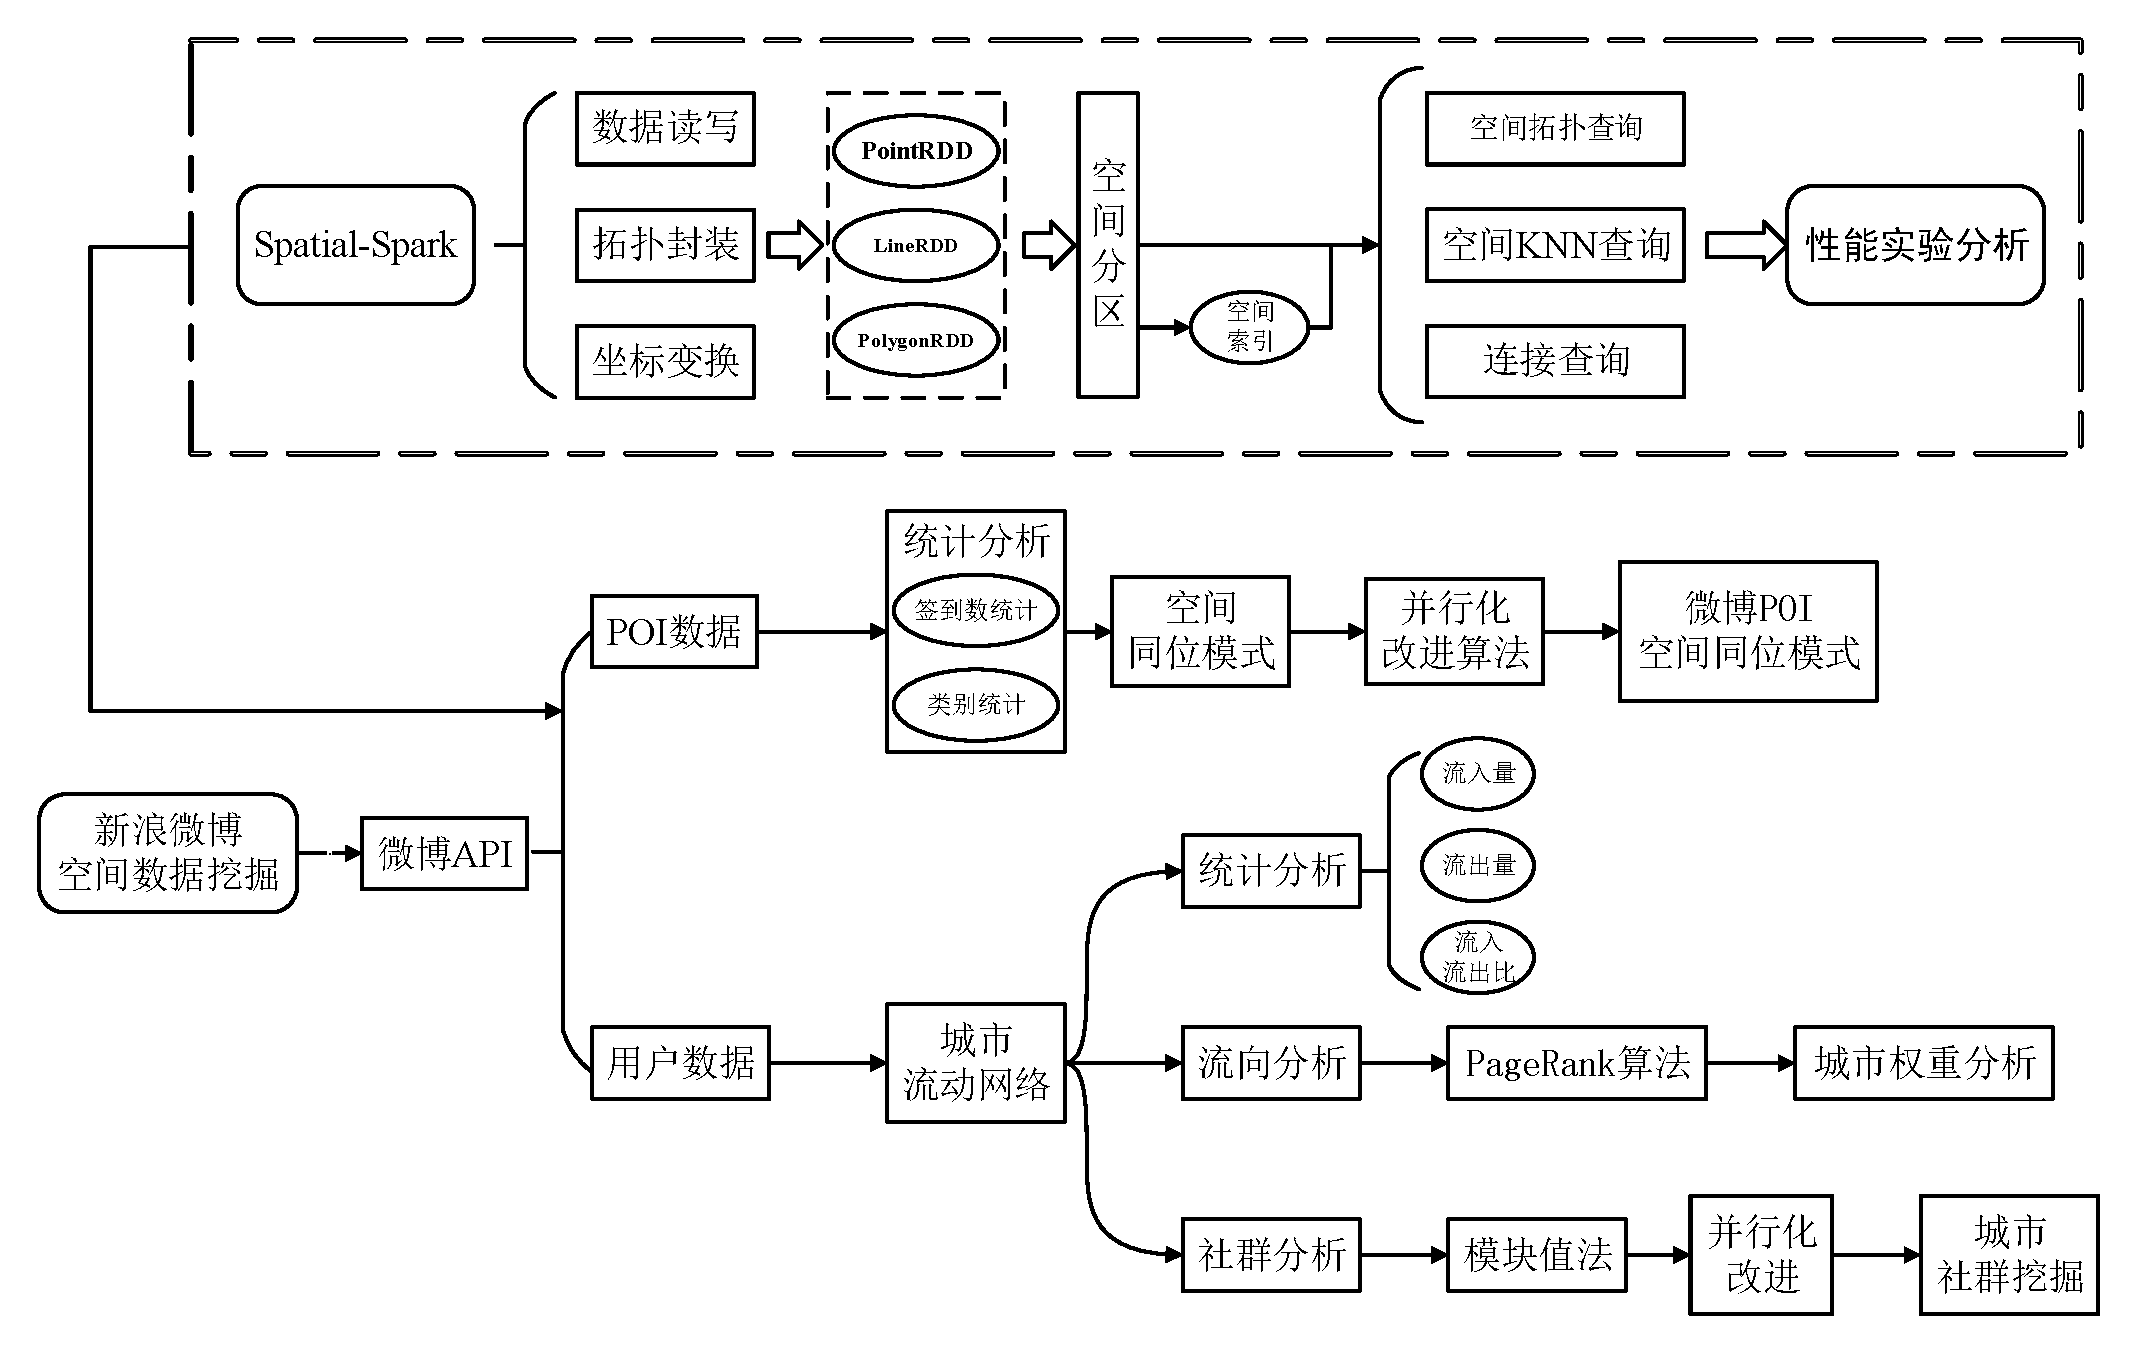
\includegraphics[height=14cm]{figures/technology_route.pdf} \\
\caption{技术路线}{Technology route}
\label{fig:thetechroute}
\end{sidewaysfigure}

\section{论文结构安排}{Contents and Structure of This Thesis}

第一章:绪论。 概要地说明了论文的研究背景及意义和国内外相关主题研究现状,
阐述了本文的工作,以及论文的主要内容和技术路线。

第二章:相关技术。重点介绍了Spark并行计算框架,空间数据挖掘相关算法和新浪微博API接口。

第三章:Spatial-Spark计算框架。设计了Spatial-Spark计算框架,对空间数据的支持,空间索引的建立和空间运算,
最后用实验比较Spatial-Spark在空间分析方面的优势。

第四章:新浪微博POI数据分析。主要包括类别统计分析和POI类别空间同位模式挖掘。

第五章:新浪微博用户流动网络分析。主要包括人口流动量统计、城市权重分析和网络社群挖掘。

第六章:总结与展望。对论文的研究内容和成果进行总结,指出了研究内容的局限性并对后期工作提出建议。
